% \subsection{Chunks, Trees and Data Integrity}

\begin{frame}[t]{\alt<5->{It's chunks all the way down...}{Chunks}}
% \begin{overlayarea}{⟨area width⟩}{⟨area height⟩}
%   ⟨environment contents⟩
% \end{overlayarea}
\begin{overlayarea}{\textwidth}{10cm}
Under the hood swarm does not deal in files but in \emph{chunks.}

\begin{itemize}
 \item<2-> All data is broken into pieces of size 4kB: ``chunks".
 \item<4-> Chunks are hashed and the hash is used as their ID/address.
 \item<5-> Chunk hashes are also packaged into 4kB chunks...
\end{itemize}

\begin{onlyenv}<1-2>
 \begin{center}
  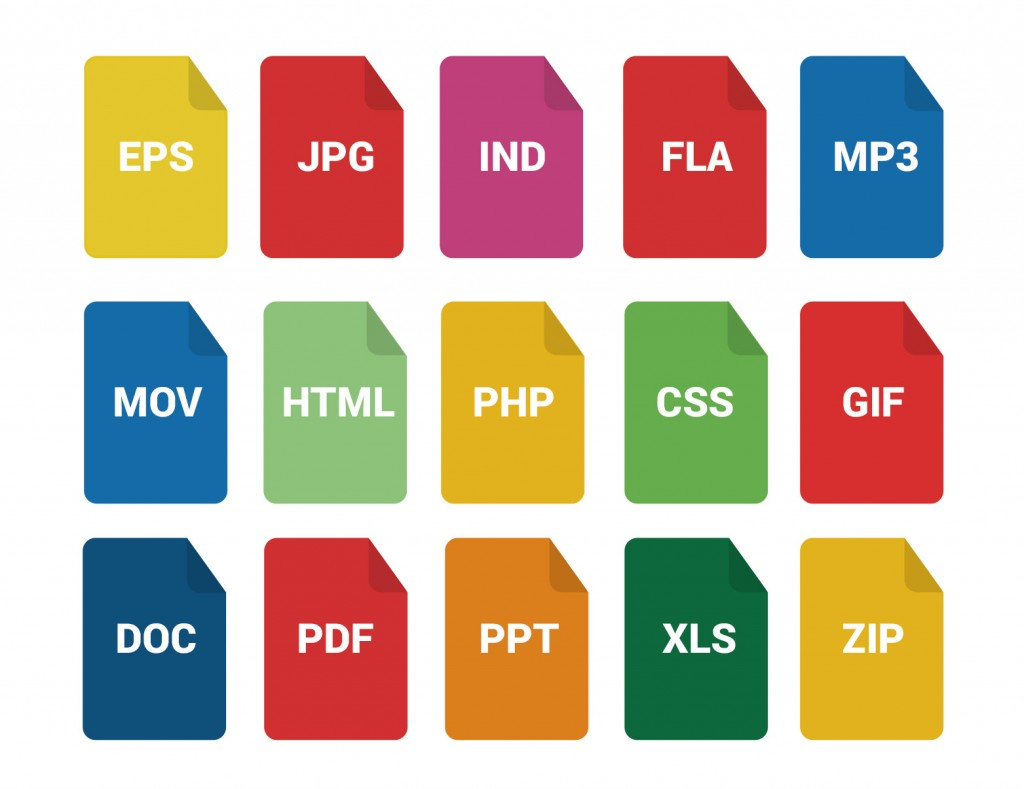
\includegraphics[width=0.4\textwidth]{devcon-files.jpg}
  \transdissolve<3>
 \end{center}
\end{onlyenv}

 \begin{center}
  \begin{tikzpicture}
   \node[chunk,visible on=<3>] at (0,0) (achunk){};
   \node[visible on=<3>] at (-1.8,0) (labeltext){A ``chunk:"};
   \node[chunk,visible on=<3->] at (-4,-3) (a){};
   \node[chunk,visible on=<3->] at (-2,-3) (b){};
   \node[chunk,visible on=<3->] at (0,-3) (c){};
   \node[chunk,visible on=<3->] at (2,-3) (d){};
   \node[chunk,visible on=<3->] at (4,-3) (e){};

   \node at (-4.2,-1.3) (dummy1) {};
   \node at (4.2,-1.7) (dummy2) {};
   \node[chunk,fit=(dummy1)(dummy2),visible on=<5>]{};

   \node[scale=0.8,draw,visible on=<4-5>] at (-4,-1.5) (ha){$h_1$}
     (a.north) edge[-,visible on=<4>] (ha.south);
   \node[scale=0.8,draw,visible on=<4-5>] at (-2,-1.5) (hb){$h_2$}
     (b.north) edge[-,visible on=<4>] (hb.south);
   \node[scale=0.8,draw,visible on=<4-5>] at (0,-1.5) (hc){$h_3$}
     (c.north) edge[-,visible on=<4>] (hc.south);
   \node[scale=0.8,draw,visible on=<4-5>] at (2,-1.5) (hd){$h_4$}
     (d.north) edge[-,visible on=<4>] (hd.south);
   \node[scale=0.8,draw,visible on=<4-5>] at (4,-1.5) (he){$h_5$}
     (e.north) edge[-,visible on=<4>] (he.south);

   \node[chunk,visible on=<6>] at (0,-1.5) {};
     \end{tikzpicture}

 \end{center}
\end{overlayarea}
\end{frame}

\begin{frame}
\begin{overlayarea}{\textwidth}{10cm}

 \begin{columns}[T]
  \begin{column}{0.5\textwidth}
  Chunks are assembled in a \textbf{Merkle Tree}.
  \small
    \begin{itemize}
     \item<1->{Files are retrievable using a single 32byte hash.}
     \item<2->{Built-in integrity protection and random access.}
     \item<3->{Merkle-proofs enable proof-of-custody schemes.}
     \item<3->{Merkle structure and BMT chunk hash enable inclusion proofs.}
    \end{itemize}

  \end{column}
  \begin{column}{0.5\textwidth}
   \only<1-2>{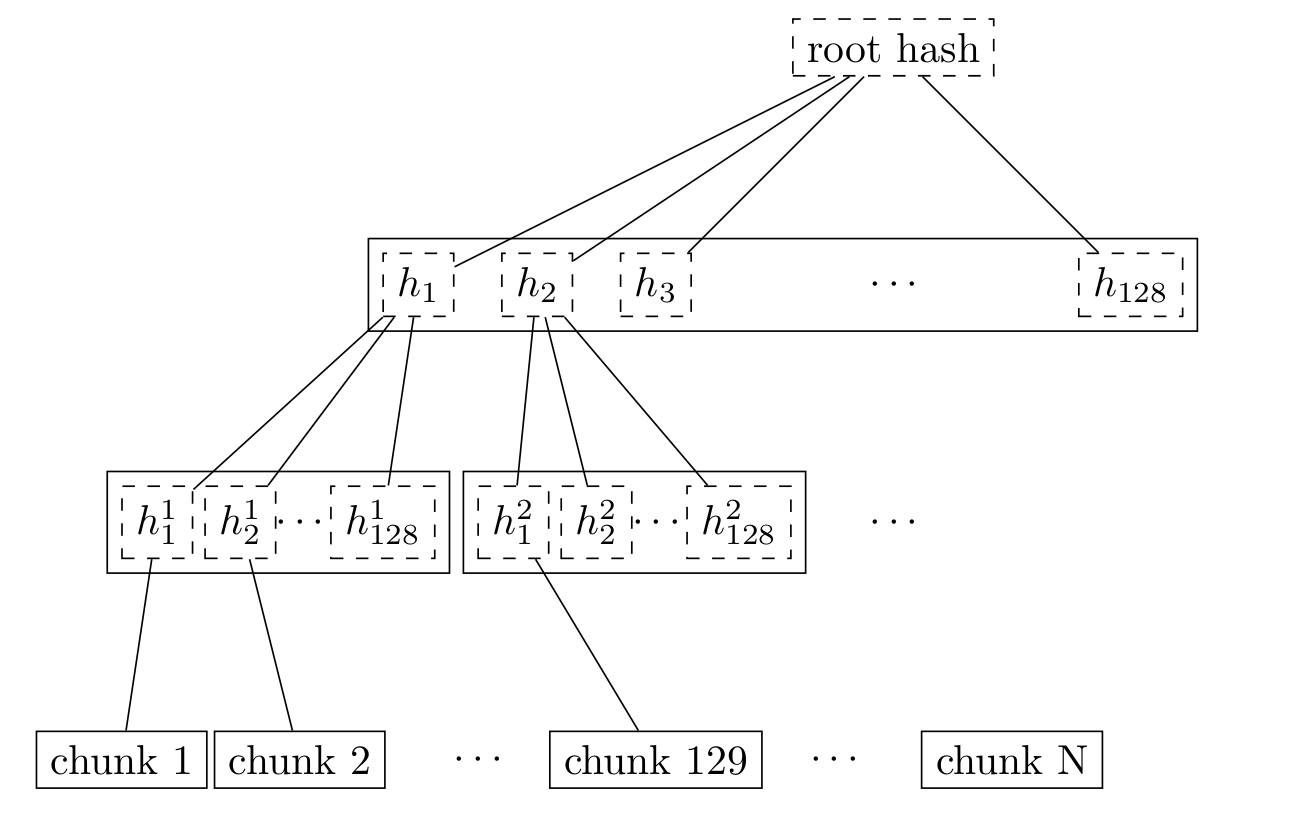
\includegraphics[width=6cm]{devcon-merkle-tree.png}}
   \only<3>{
   \begin{tikzpicture}
    \node[scale=0.4] {
    \documentclass[border=2pt,draw]{standalone}
\usepackage{tikz}
\usetikzlibrary{fit}
\begin{document}

\tikzset{
level/.style={
  sibling distance={(width("$H^126$")+4pt)},
  level distance=15mm,
  line width=.5pt,
},
mtnode/.style={
  minimum width={width("$H^126$")+2pt},
  minimum height={.7cm},
  inner sep=2pt,
  outer sep=2pt,
  rectangle,
  rounded corners=1pt,
  draw,
},
% edge from parent/.style={draw=none},
mtedge/.style={grow=down,draw=none,<-, edge from parent/.style={draw}},
link/.style={draw=none, edge from parent/.style={draw=none}},
mtedgeadj/.style={mtedge, shorten >=10pt  },
mpedge/.style={mtedge, line width=.7pt,densely dashed},
ellip/.style={draw,loosely dotted, shorten >=5mm, thick,<-, edge from parent/.style={draw}},
bubble/.style={minimum height={1cm}, draw=none, align=center},
data/.style={mtnode, fill=gray!50},
mppath/.style={mtnode,dashed,line width=.7pt,fill=gray!30},
mpext/.style={mtnode,line width=.7pt,fill=gray!40},
mpdata/.style={data,line width=.7pt,fill=gray!70},
mpdataext/.style={data,line width=.7pt,fill=gray!80},
}

\begin{tikzpicture}
                  % level 7
\node[mtnode] (root) {$H^7_0$}
                  % level 6
  child[<-,grow=right,level distance=3cm] { node[bubble] (ash) {root-hash}  }
  % child[link,grow=left,level distance=5cm] { node[bubble] (ash) {audit secret}  }
  child { node[mppath] (6-0) {$H^6_0$}   % 0
                  % level 5
    child { node[mppath] (5-0) {$H^5_0$}          % 0
      % child[mpedge]
                  % level 4
                  % mppath goes the other way
      child { node[mpext] (4-0) {$H^4_0$}
        % % child[mtedgeadj]
                  % level 3
        child { node[mtnode] (3-0) {$H^3_0$}
              % level 2
          child { node[mtnode] (2-0) {$H^2_0$}
                % level 1
            child { node[mtnode] (1-0) {$H^1_0$}
                % level 0
              child { node[mtnode] (0-0) {$H^0_0$}
                % data level
                child[mtedge] { node[data] (c-0) {$c_0$} }
              }
              % % child[mtedgeadj]
              child { node[mtnode] (0-1) {$H^0_1$}
                % data level
                child[mtedge] { node[data] (c-1) {$c_1$} }
              }
                % level 0
            }
                % level 1
            % child[mtedgeadj]
            child { node[mtnode] {$H^1_{1}$} child[ellip] }
          }
                % level 2
          % child[mtedgeadj]
          child { node[mtnode] {$H^2_{1}$} child[ellip] }
        }
                % level 3
        % child[mtedgeadj]
        child { node[mtnode] {$H^3_{1}$} child[ellip] }
      }
                % level 4
      child[missing]
      child[missing]
      child { node[mppath] (4-1) {$H^4_1$}                 % 1
                % level 3
        child { node[mpext] (3-4) {$H^3_4$} child[ellip] }
        % child[mpedge]
        child { node[mppath] (3-5) {$H^3_5$}  % 1
                % level 2
          % child[mpedge]
          child { node[mppath] (2-10) {$H^2_{10}$}           % 0
                % level 1
            child { node[mpext] (1-21) {$H^1_{21}$} child[ellip] }
            % child[mpedge]
            child { node[mppath] (1-22) {$H^1_{22}$}         % 1
                % level 0
              child { node[mppath] (0-42) {$H^0_{42}$}       % 0
                % data level
                child[mtedge] { node[mpdata] (c-42) {$c_{42}$} }    % <- pivot
              }
                % level 0
              % child[mpedge]
              child { node[mpext] (0-43) {$H^0_{43}$}
                % data level
                child[mtedge] { node[mpdataext] (c-43) {$c_{43}$} }    % <- neighbo
              }
                % level 0
            }
                % level 1
          }
                % level 2
          % child[mpedge]
          child { node[mpext] (2-11) {$H^2_{11}$} child[ellip] }
        }
                % level 3
        % child[missing]
      }
                % level 4
    }
                % level 5
    child[missing]
    % child[mpedge]
    child[missing]
    child { node[mpext] (5-1) {$H^5_1$} child[ellip] }
  }
                % level 6
  child[missing]
  child[missing]
  % child[mtedgeadj]
  child[missing]
  child  { node[mpext] (6-1) {$H^6_1$}
                % level 5
    child { node[mtnode] (5-2) {$H^5_2$} child[ellip] }
    child[missing]
    % child[mtedgeadj]
    child { node[mtnode] (5-3) {$H^5_3$}
                % level 4
      child { node[mtnode] {$H^4_{6}$} child[ellip] }
      % child[mtedgeadj]
      child { node[mtnode] (4-7) {$H^4_7$}
                % level 3
        child { node[mtnode] {$H^3_{14}$} child[ellip] }
        % child[mtedgeadj]
        child { node[mtnode] (3-15) {$H^3_{15}$}
                % level 2
          child { node[mtnode] {$H^3_{30}$} child[ellip] }
          % child[mtedgeadj]
          child { node[mtnode] (2-31) {$H^2_{31}$}
                % level 1
            child { node[mtnode] {$H^1_{62}$} child[ellip] }
            % child[mtedgeadj] {node {}}
            child { node[mtnode] (1-63) {$H^1_{63}$}
                % level 0
              child { node[mtnode] (0-126) {$H^0_{126}$}
                child[mtedge] { node[data] (c-126) {$c_{126}$} }
              }
              % child[mtedgeadj]
              child { node[mtnode] (0-127) {$H^0_{127}$}
                child[mtedge] { node[data] (c-127) {$c_{127}$} }
              }
                % 0
            }
                % 1
          }
                % 2
        }
                % 3
      }
                % 4
    }
               % 5
  }
               % 6
 ;
\end{tikzpicture}
\end{document}
    };
   \end{tikzpicture}
   }
   \only<4>{
     \begin{tikzpicture}
      \node[scale=0.6] {
         \begin{tikzpicture}
	  \node[draw,dashed] (root) at (5,3) {hash of chunk $h_1$ - $h_{128}$};
	  \node[draw,dashed] (h1) at (1,1) {$h_1$};
	  \node[draw,dashed] (h2) at (2,1) {$h_2$};
	  \node[draw,dashed] (h3) at (3,1) {$h_3$};
	  \node (dots) at (5,1) {$\cdots$};
	  \node[draw,dashed] (h128) at (7,1) {$h_{128}$};
	  % \node[draw,fit=(h1) (h2) (h3) (dots) (h128)]{};
	  \draw (root) -- (h1);
	  \draw (root) -- (h2);
	  \draw (root) -- (h3);
	  \draw (root) -- (h128);
      \end{tikzpicture}
      };
      \end{tikzpicture}
      }
  \end{column}
 \end{columns}

\end{overlayarea}
\end{frame}

\begin{frame}{Manifests}
 We can take this one step further, be tying together various swarm assets under a new root-hash by generating a new tree: A \textbf{Manifest}.\\
 \begin{block}{A Swarm Manifest...}
  ...is a Merkle tree whose leaves are root-hashes of other swarm assets (files, collections, manifests, chunks...)
 \end{block}
 The only difference between this and the chunk-tree of a file, is that it is not balanced and has metadata.
\end{frame}

\begin{frame}
 For example, \uncover<2->{the Swarm landing page
 \begin{center}
  \texttt{swarm-gateways.net/bzz:/swarm/}
 \end{center}
 }
 \end{frame}

\begin{frame}
 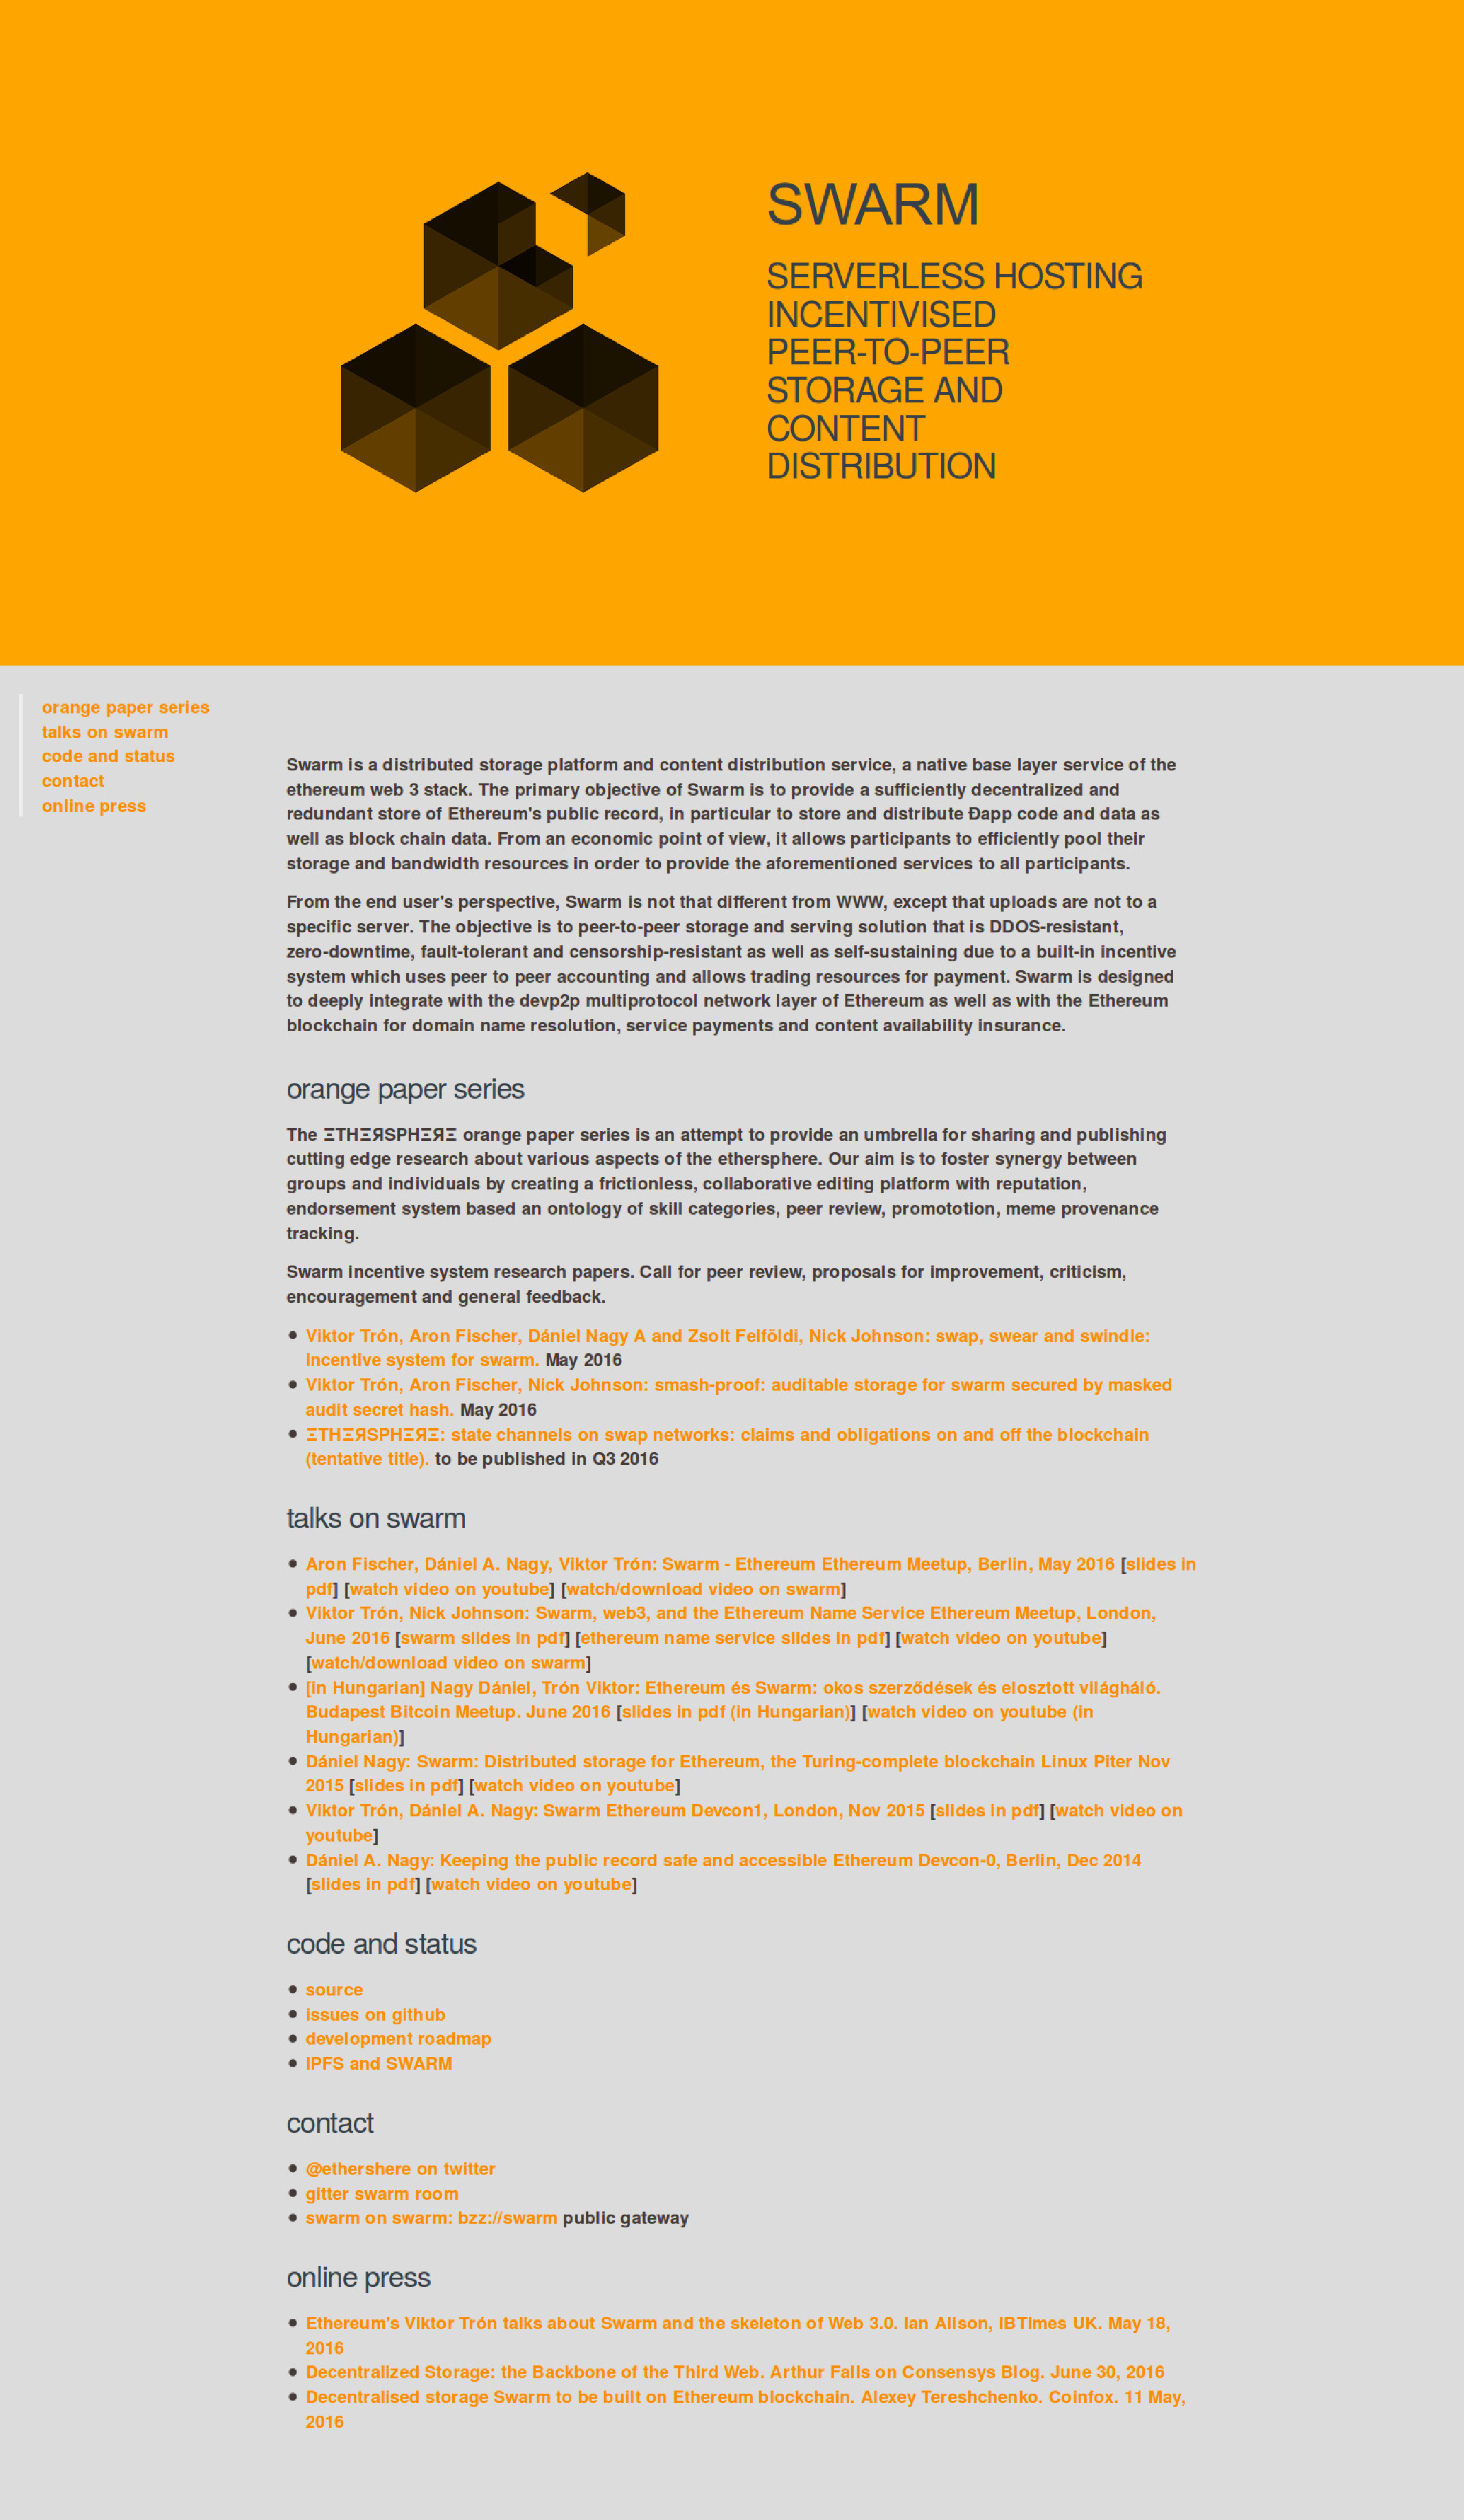
\includegraphics[width=0.8\textwidth]{devcon-swarmsite.pdf}
\end{frame}

\begin{frame}[fragile]
\frametitle{Manifests}
 ...is loaded from this 4-entry manifest:\\
\tiny
\begin{semiverbatim}
\{"entries":[\{
"path":"Swarm_files/",
"hash":"0294e48456a49fe7c02162c83b068075ff9ae6aaafb46439dba32da7de548379",
"contentType":"application/bzz-manifest+json",
"status":0\},
\{"path":"ethersphere/orange-papers/"...
\{"path":"i"...
\{"path":"talks/"...
\{"path":"",
"hash":"6fac0b0c1f118f7f383792c0f01c80d1b2dc94f0e166d62ff4f999a926e9d94a",
"contentType":"text/html;charset=utf-8","status":0\}]\}\end{semiverbatim}
\uncover<2->{\small
 Manifests translate a URL path into swarm hashes (URL defines manifest merkle-tree traversal).\\[2mm]
 When combined with the Ethereum Name Service (ENS) to register a name for the manifest's own root hash, we can \textbf{serve any and all swarm data directly to your browser using human readable names}.
}
\end{frame}

% \begin{subsection}{Example: Swarm File Manager}
 \begin{frame}
  With manifests, you can navigate swarm just like you would navigate your own filesystem.\\
  \uncover<2->{Let us open the swarm landing page in the swarm file manager:\\}
  \uncover<3->{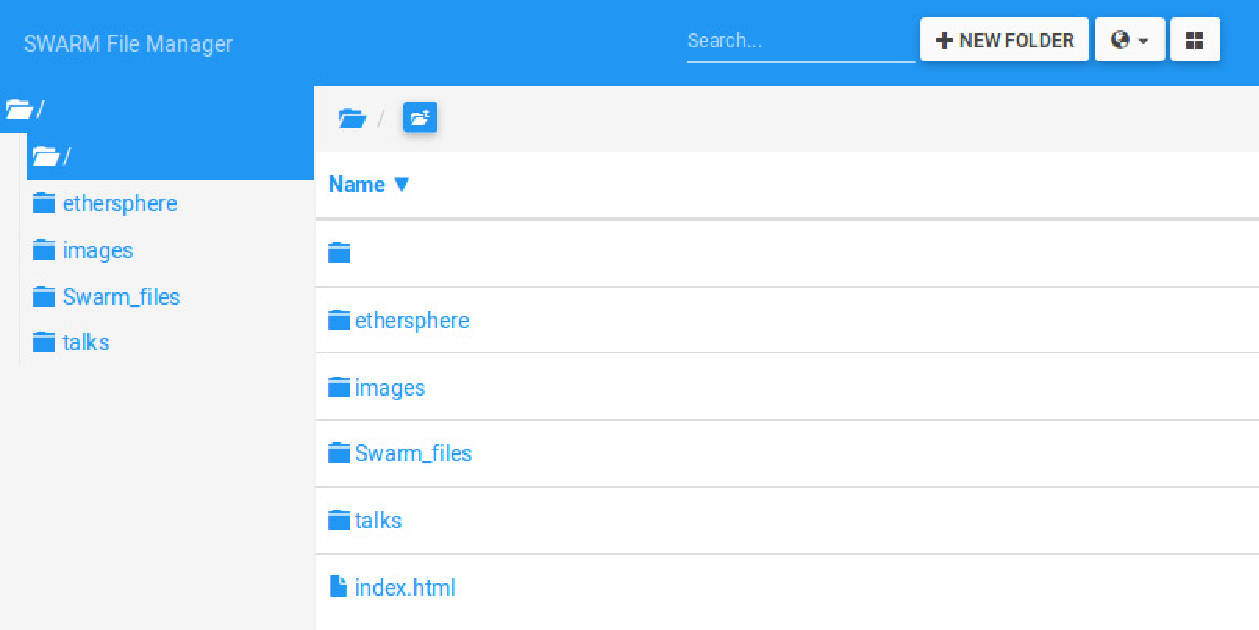
\includegraphics[width=11cm]{devcon-swarmfilemanager.pdf}}
 \end{frame}
% \end{subsection}


% \begin{subsection}{Manifest Uses}

\begin{frame}

\begin{block}{Using Manifests...}
\begin{itemize}
 \item Two-way translation possible from directories to manifests
  \begin{itemize}
   \item Filesystem API
   \item Dropbox, rsync, ...
   \item Filesystem driver (fuse)
  \end{itemize}
 \item Only root hashes must be registered (ENS) on blockchain. Beyond this the whole site is integrity protected.
 \item Metadata for any manifest entry can include
    \begin{itemize}
      \item copyright information
      \item access control
      \item payment triggers
      \item auto-play continuation
      \item subscription information
      \item database layout info
    \end{itemize}
 \item Version control system (mango = git over swarm)
\end{itemize}
\end{block}

\end{frame}
% \end{subsection}
